\documentclass[a4paper, 12pt]{article}

\usepackage{geometry}
\geometry{left=2cm, right=2cm, top=2cm, bottom=2cm}

\usepackage{cmap}
\usepackage{mathtext} 
\usepackage[T2A]{fontenc}
\usepackage[utf8]{inputenc}
\usepackage[english,russian]{babel}	

\usepackage{amsfonts,amssymb,amsthm,mathtools}
\usepackage{amsmath}
\usepackage{icomma} 

\usepackage{graphicx} 
\graphicspath{{picturies/}}
\usepackage{wrapfig}

\usepackage{array,tabularx,tabulary,booktabs}
\usepackage{longtable}
\usepackage{multirow}

\usepackage{caption}
\captionsetup{labelsep=period}

\renewcommand{\phi}{\varphi}
\newcommand{\eps}{\varepsilon}
\newcommand{\parag}[1]{\paragraph*{#1:}}

\newcounter{Points}
\setcounter{Points}{1}
\newcommand{\point}{\arabic{Points}. \addtocounter{Points}{1}}

\author{Радькин Кирилл, Б01-005}
\date{14.05.22}
\title{Лабораторная работа 4.3.2. Дифракция света на ультразвуковой волне в жидкости.}

\begin{document}
    \maketitle

    \textbf{\\Цель работы:} изучение дифракции света на синусоидальной акустической решетке и наблюдение фазовой решетки методом темного поля

    \textbf{\\В работе используются:} оптическая скамья, осветитель, два длиннофокусных объектива, кювета с жидкостью, кварцевый излучатель с микрометрическим винтом, генератор звуковой частоты, линза, вертикальная нить на рейтере, микроскоп.

    \textbf{\\Экспериментальная установка:}

    \begin{figure}[!h]
        \centering
        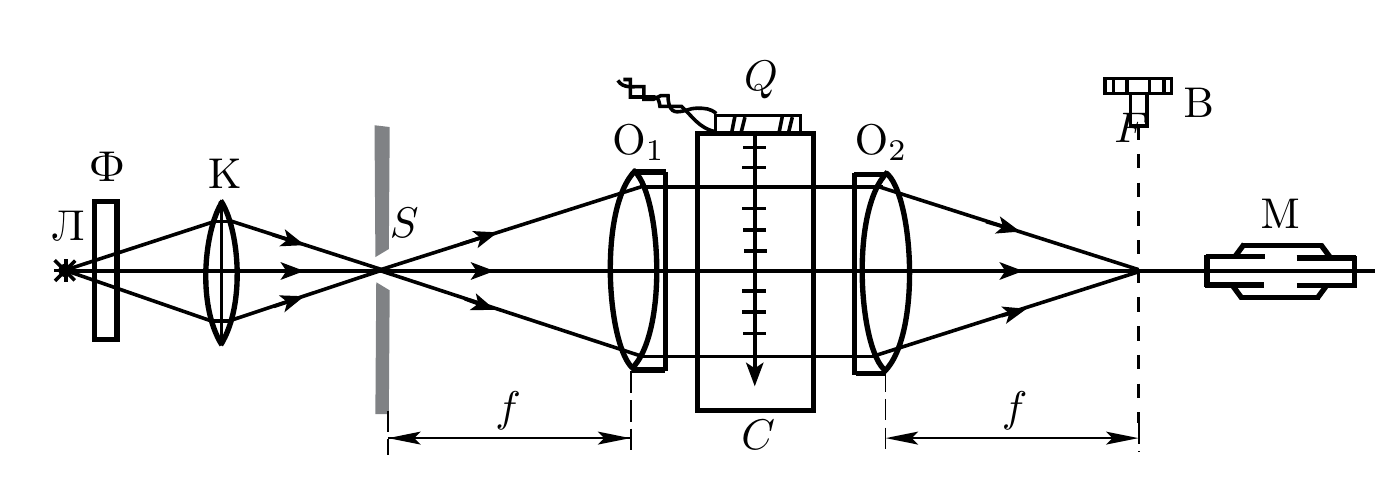
\includegraphics[scale = 0.7]{shema1.png}
        \caption{Схема для наблюдения дифракции на акустической решетке}
        \label{pic1}
    \end{figure}

    \begin{figure}[!h]
        \centering
        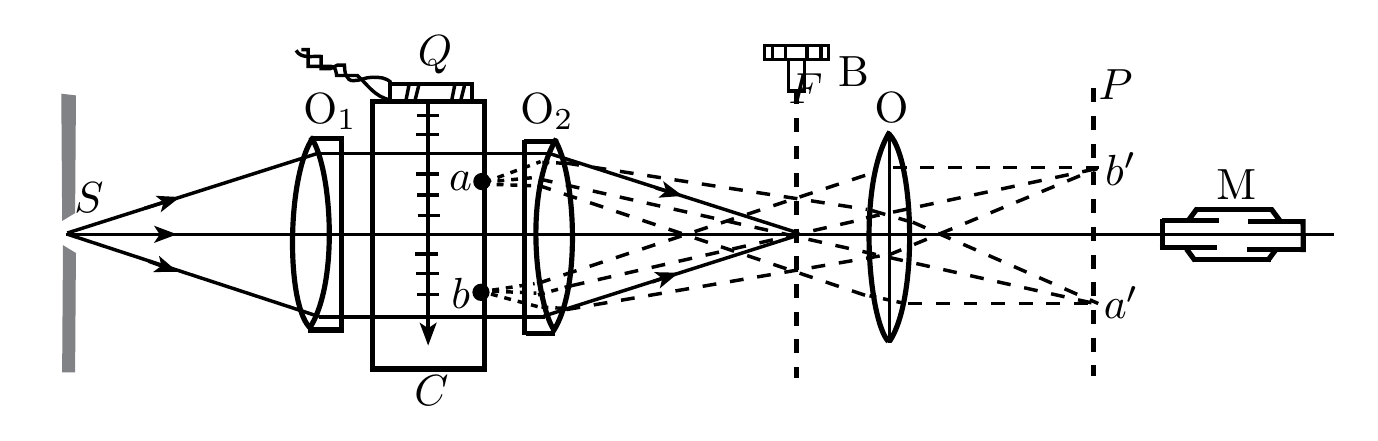
\includegraphics[scale = 0.7]{shema2.png}
        \caption{Схема для наблюдения дифракции методом темного поля}
        \label{pic2}
    \end{figure}

    \textbf{\\Теоретическая справка:}

    \begin{itemize}
        \item Длина $\Lambda$ ультразвуковой волны определяется по формуле
            \begin{equation}
                \label{eq1}
                \Lambda\sin{\Theta_m}~=~m\lambda 
            \end{equation}

            В силу малости углов:
            \begin{equation}
                \label{eq2}
                l_m~=~mf\dfrac{\lambda}{\Lambda}
            \end{equation}

            где $l_m$~---~измеренное на опыте линейное расстояние между m-м и нулевым максимумами, а f~---~фокусное расстояние объектива $O_2$.

        \item Скорость $v$ распространения звука в воде ($\nu$~---~частота кварцевого излучателя):
            \begin{equation}
                \label{eq3}
                v~=~\Lambda \nu
            \end{equation}

        \item Длина волны в воде для метода темного поля:
            \begin{equation}
                \label{eq4}
                \dfrac{\Lambda}{2}~=~T C
            \end{equation}

            где $T$~---~период решетки (в делениях), а $C$~---~цена деления.
    \end{itemize}

    \textbf{\\Ход работы:}

    \begin{enumerate}
        \item Настроим установку, получим четкую дифракционную картину. Запишем фокусные расстояния объективов $O_1$ и $O_2$ ($f~=30$ см)
        \item Для выбранных частот излучателя определим положения $x_m$ шести-восьми дифракционных максимумов (одно деление~---~4 мкм):
        
            \begin{tabular}{|c|c|c|c|c|c|c|c|c|c|c|c|c|} \hline
                $f$ & \multicolumn{3}{|c|}{1 МГц} & \multicolumn{3}{|c|}{2 МГц} & \multicolumn{3}{|c|}{3 МГц} & \multicolumn{3}{|c|}{3.5 МГц}\\ \hline
                $n$ & -1 & 0 & 1 & -1 & 0 & 1 & -1 & 0 & 1 & -1 & 0 & 1 \\ \hline
                $x$, дел. & 108 & 77 & 48 & 144 & 83 & 11 & 272 & 180 & 79 & 284 & 174 & 63 \\ \hline
            \end{tabular}

        \item Построим графики $x_m$ от $m$ для каждой частоты (см. рис. \ref{g1}, \ref{g2}, \ref{g3}, \ref{g4}):

        \item Рассчитаем длину волны $\Lambda$ по формуле \ref{eq2}:
        
            \begin{tabular}{|c|c|c|c|c|} \hline
                $L$, мкм & $1600 \pm 53$ & $685 \pm 42$ & $497 \pm 22$ & $434 \pm 27$ \\ \hline
                $f$, МГц & 1 & 2 & 3 & 3.5 \\ \hline
            \end{tabular}

        \item Рассчитаем скорость звука в воде по формуле \ref{eq3}:
            
            \begin{tabular}{|c|c|c|c|c|} \hline
                $v$, м/c & $1600 \pm 53$ & $1371 \pm 86$ & $1492 \pm 65$ & $1520 \pm 93$ \\ \hline
                $f$, МГц & 1 & 2 & 3 & 3.5 \\ \hline
            \end{tabular}

            В среднем отличается от теоретического значения (1490 м/с) на $\approx 3\%$

        \item Перейдем к методу темного поля. Введем в поле зрения вертикальную проволочку, опустим в воду пластинку с делениями.
        \item Определим цену деления окулярной шкалы: 10 дел. $\approx$ 1 мм
        \item Закроем центральный максимум вертикальной нитью.
        \item Определим длину волны в воде. Для этого посчитаем период решетки:
        
            \begin{tabular}{|c|c|c|} \hline
                $f$ & $1.2$ МГц & $1.07$ Мгц \\ \hline
                $T$, дел. & 6.0 & 7.2 \\ \hline                
            \end{tabular}

            Далее, используя формулу \ref{eq4} посчитаем $\Lambda$:

            \begin{tabular}{|c|c|c|} \hline
                $f$ & $1.2$ МГц & $1.07$ Мгц \\ \hline
                $\Lambda$, мкм. & $1200 \pm 20$ & $1440 \pm 20$ \\ \hline                
            \end{tabular}
        \item Определим, используя найденные $\Lambda$ скорость звука в воде:
        
            \begin{tabular}{|c|c|c|} \hline
                $f$ & $1.2$ МГц & $1.07$ Мгц \\ \hline
                $v$, м/с & $1440 \pm 24$ & $1540 \pm 21$ \\ \hline                
            \end{tabular}

            В среднем отличается от теоретического значения (1490 м/с) на $\approx 1.5\%$
    \end{enumerate}

    \begin{figure}[!h]
        \centering
        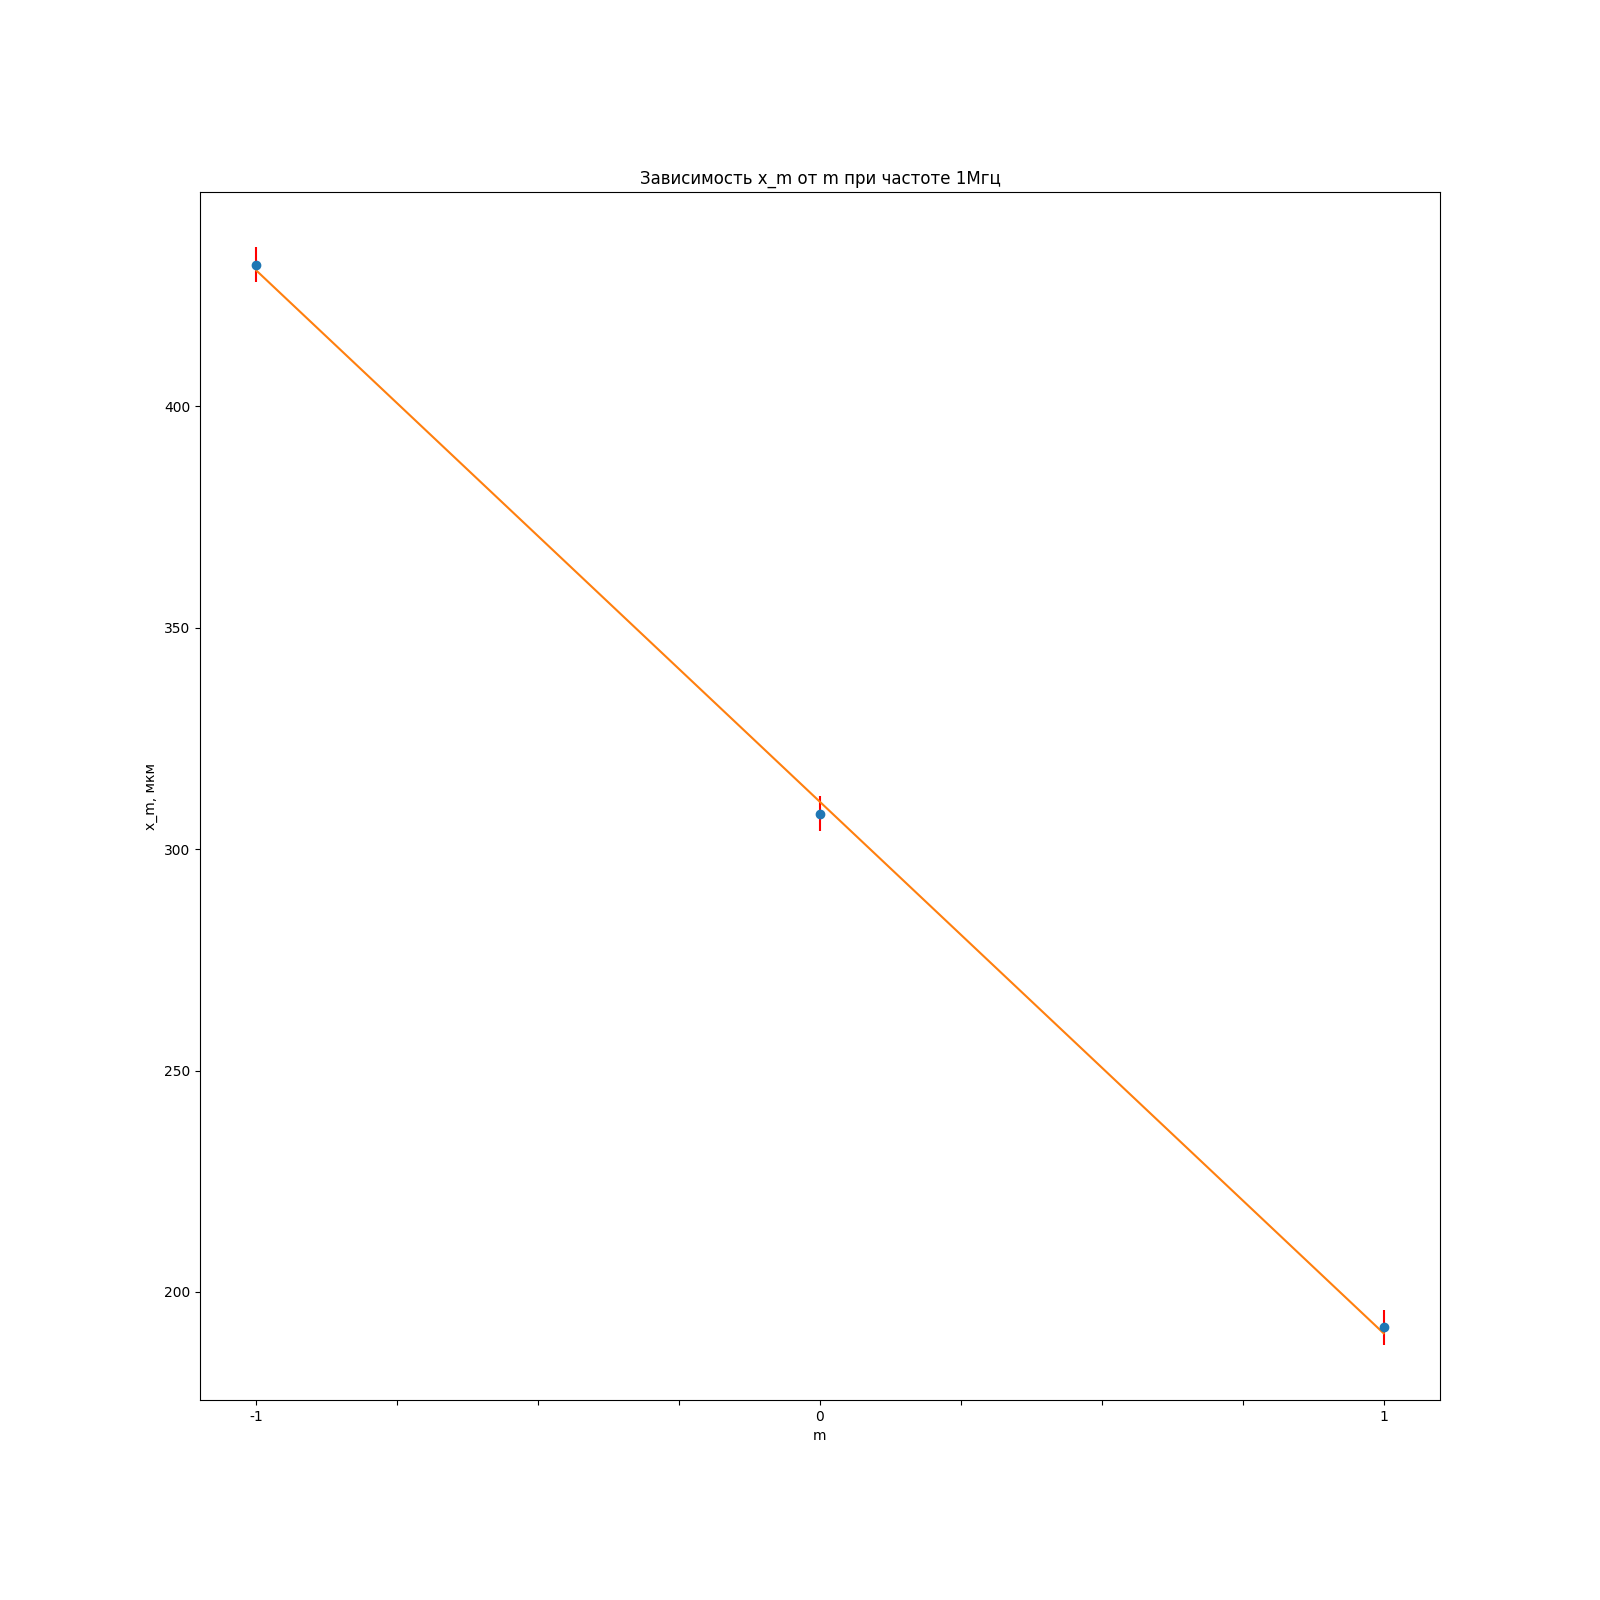
\includegraphics[scale = 0.4]{graph1.png}
        \caption{$f~=~1$ МГц}
        \label{g1}
    \end{figure}

    \begin{figure}[!h]
        \centering
        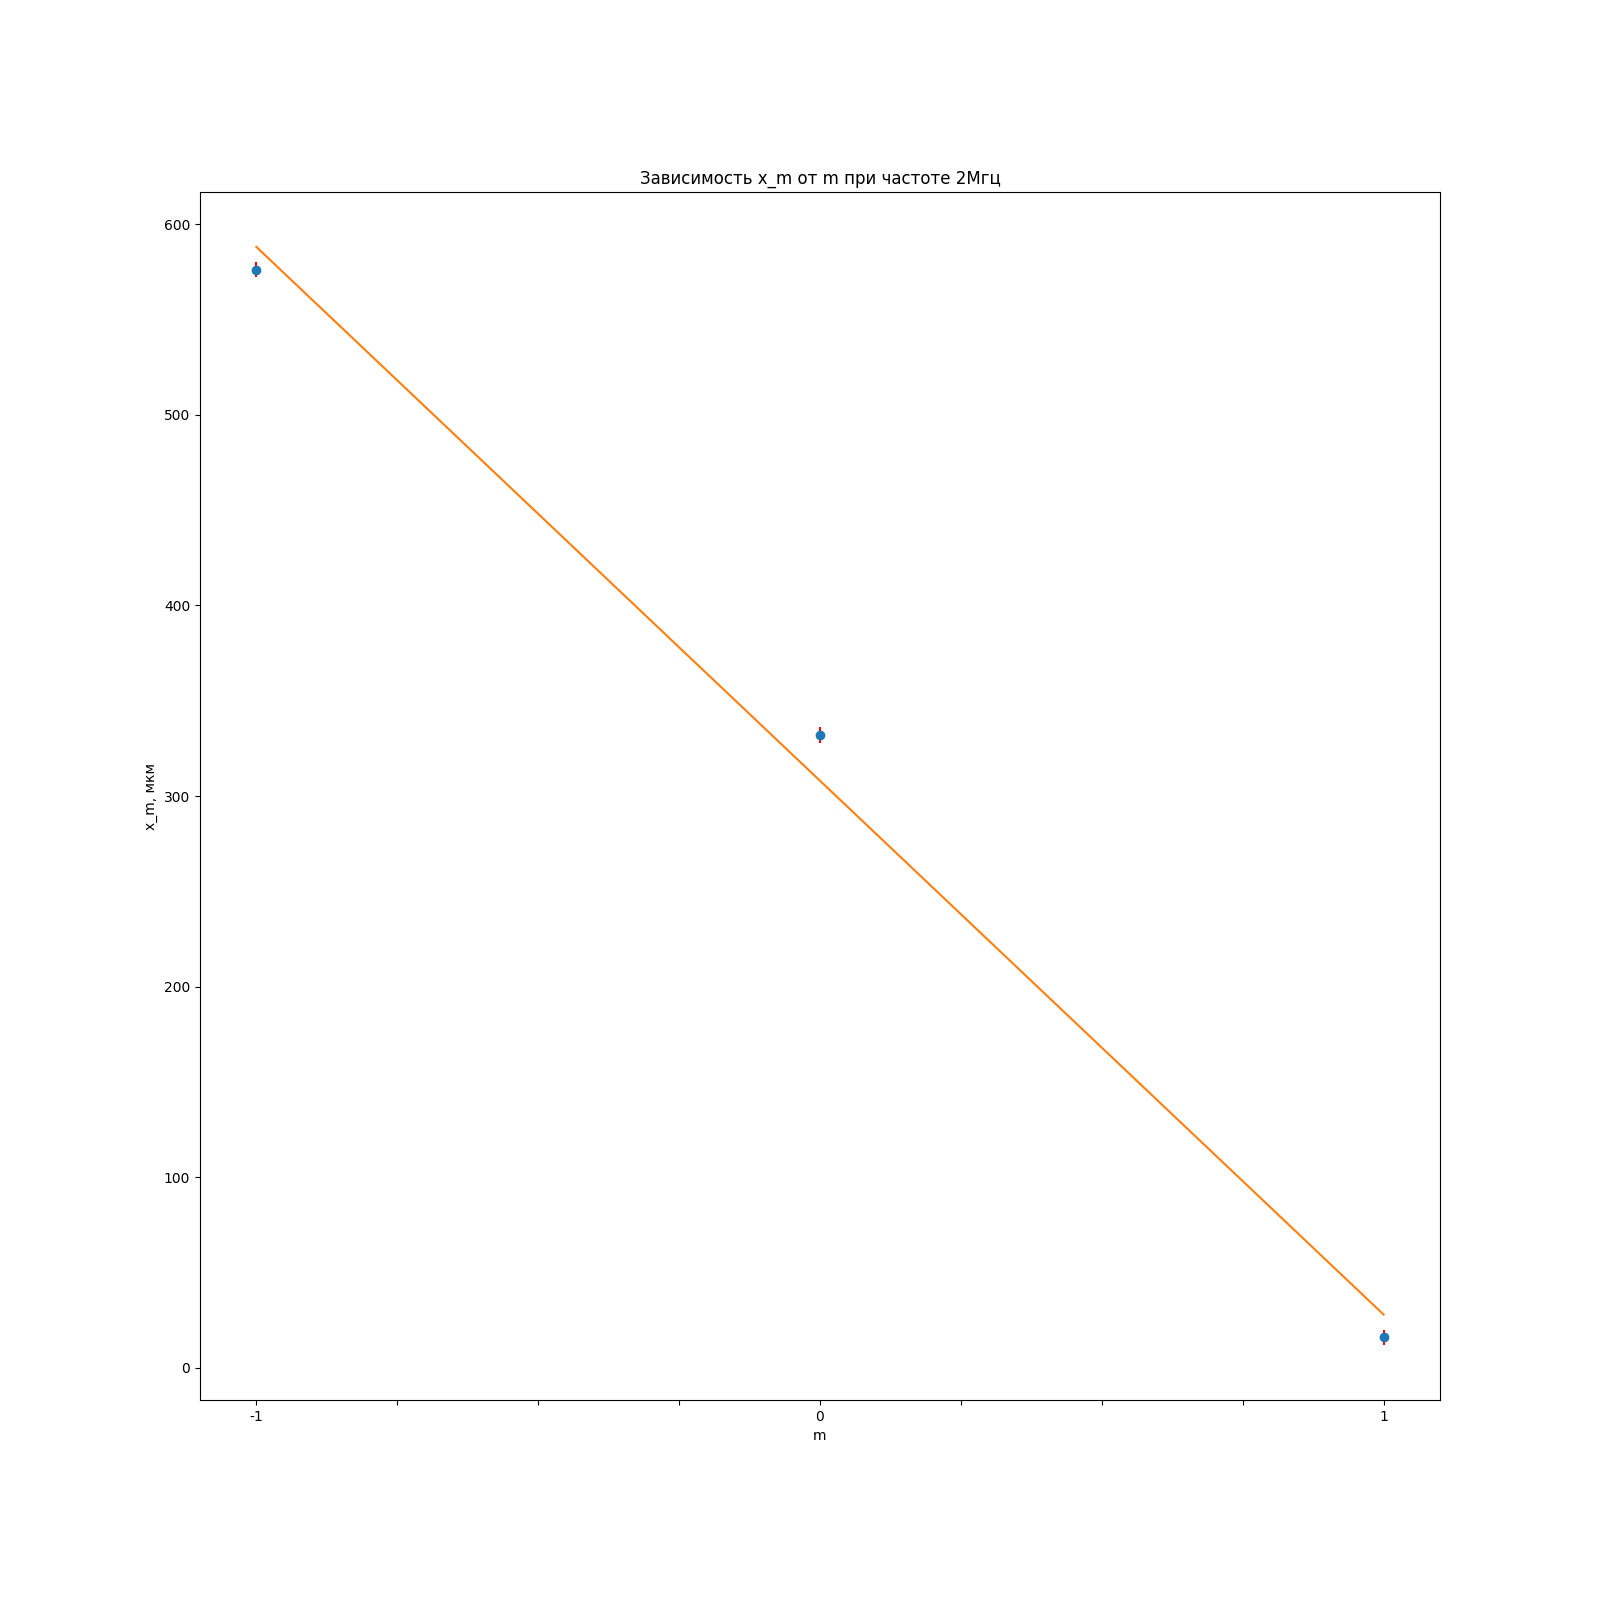
\includegraphics[scale = 0.4]{graph2.png}
        \caption{$f~=~2$ МГц}
        \label{g2}
    \end{figure}

    \begin{figure}[!h]
        \centering
        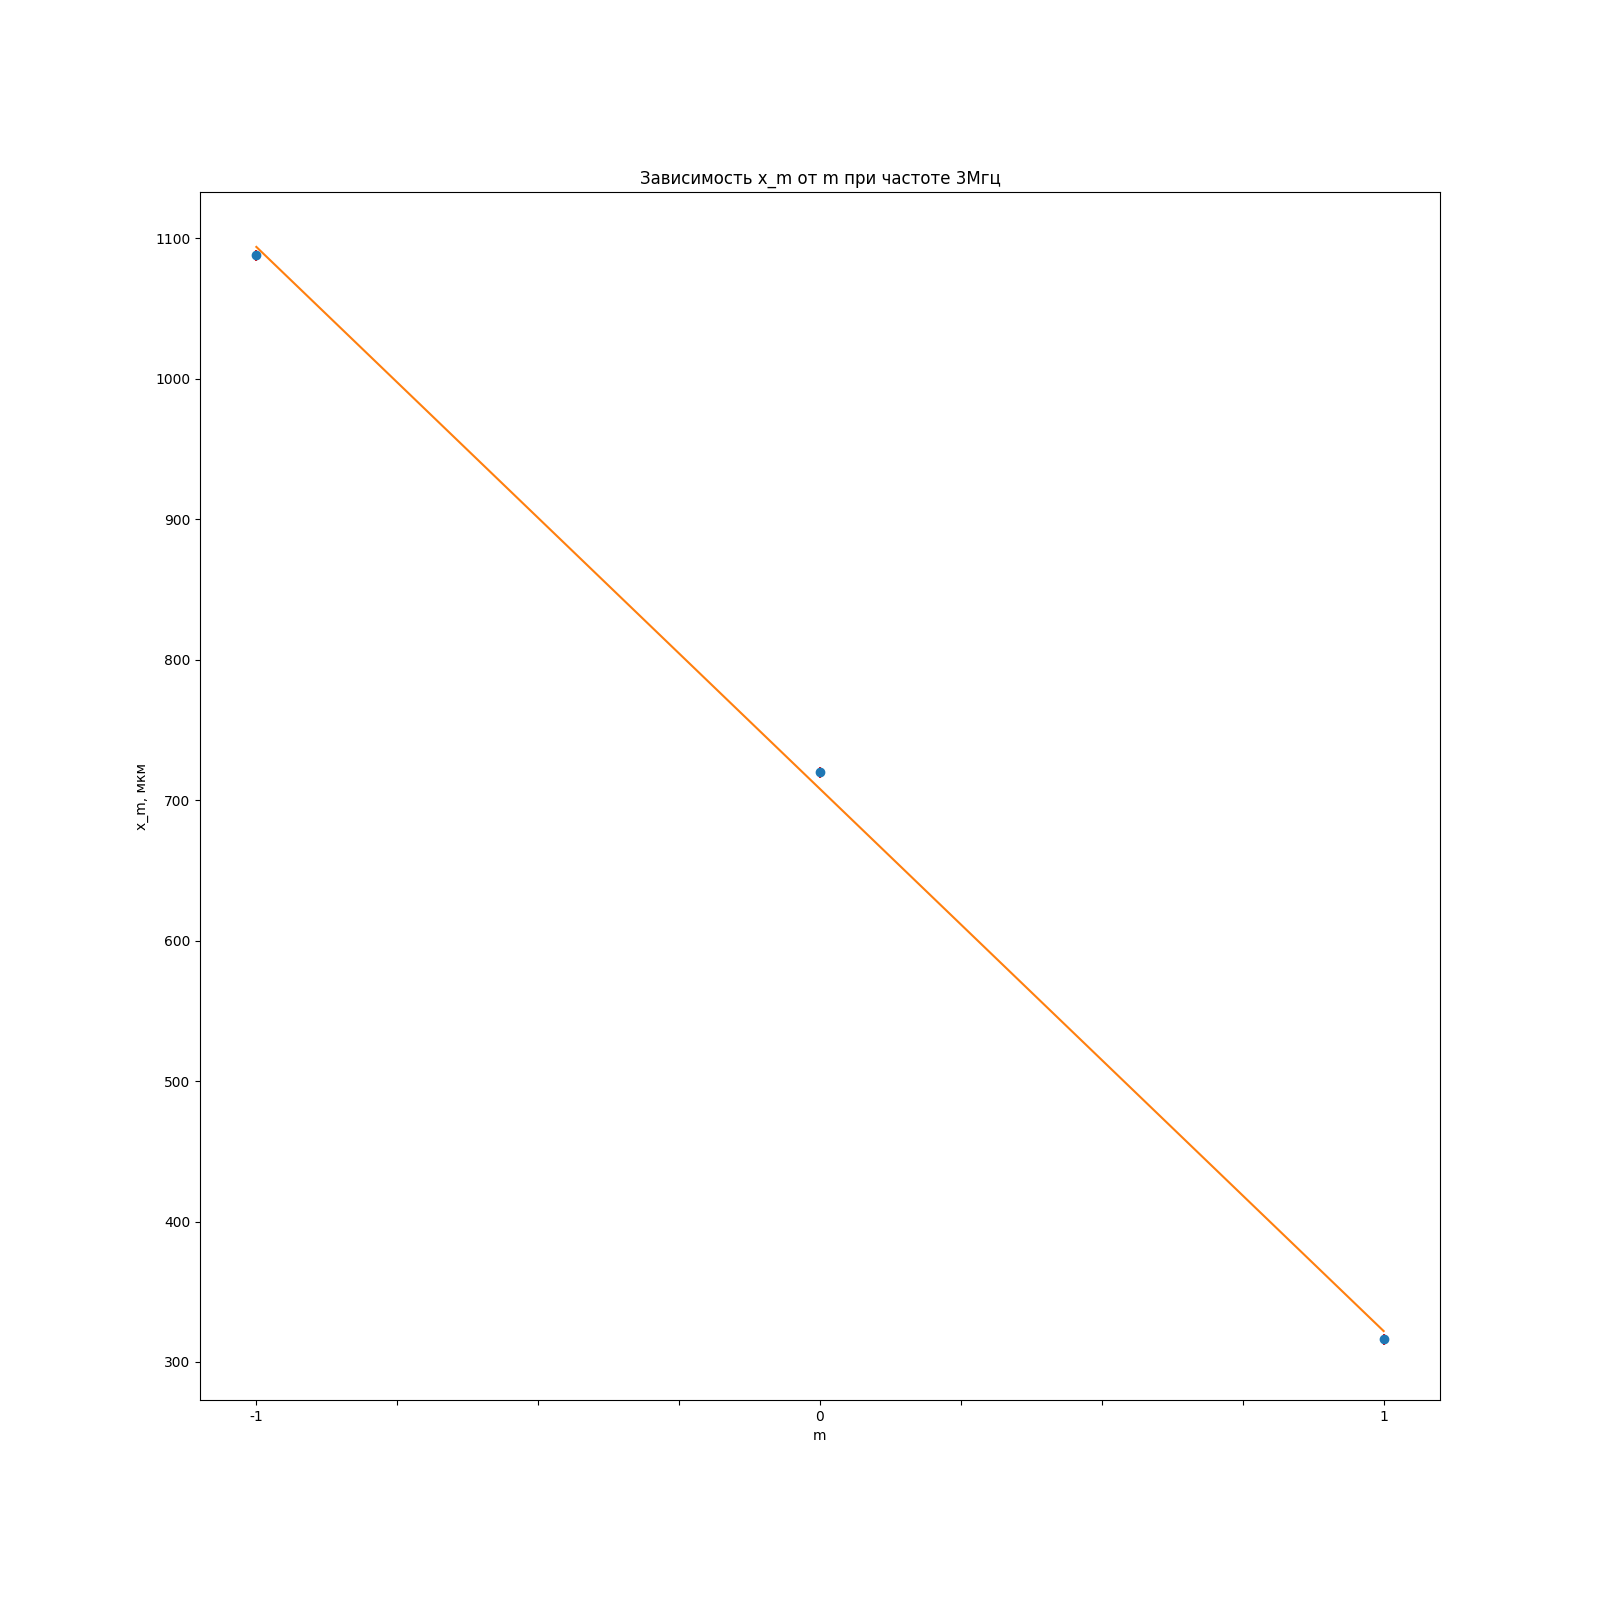
\includegraphics[scale = 0.4]{graph3.png}
        \caption{$f~=~3$ МГц}
        \label{g3}
    \end{figure}

    \begin{figure}[!h]
        \centering
        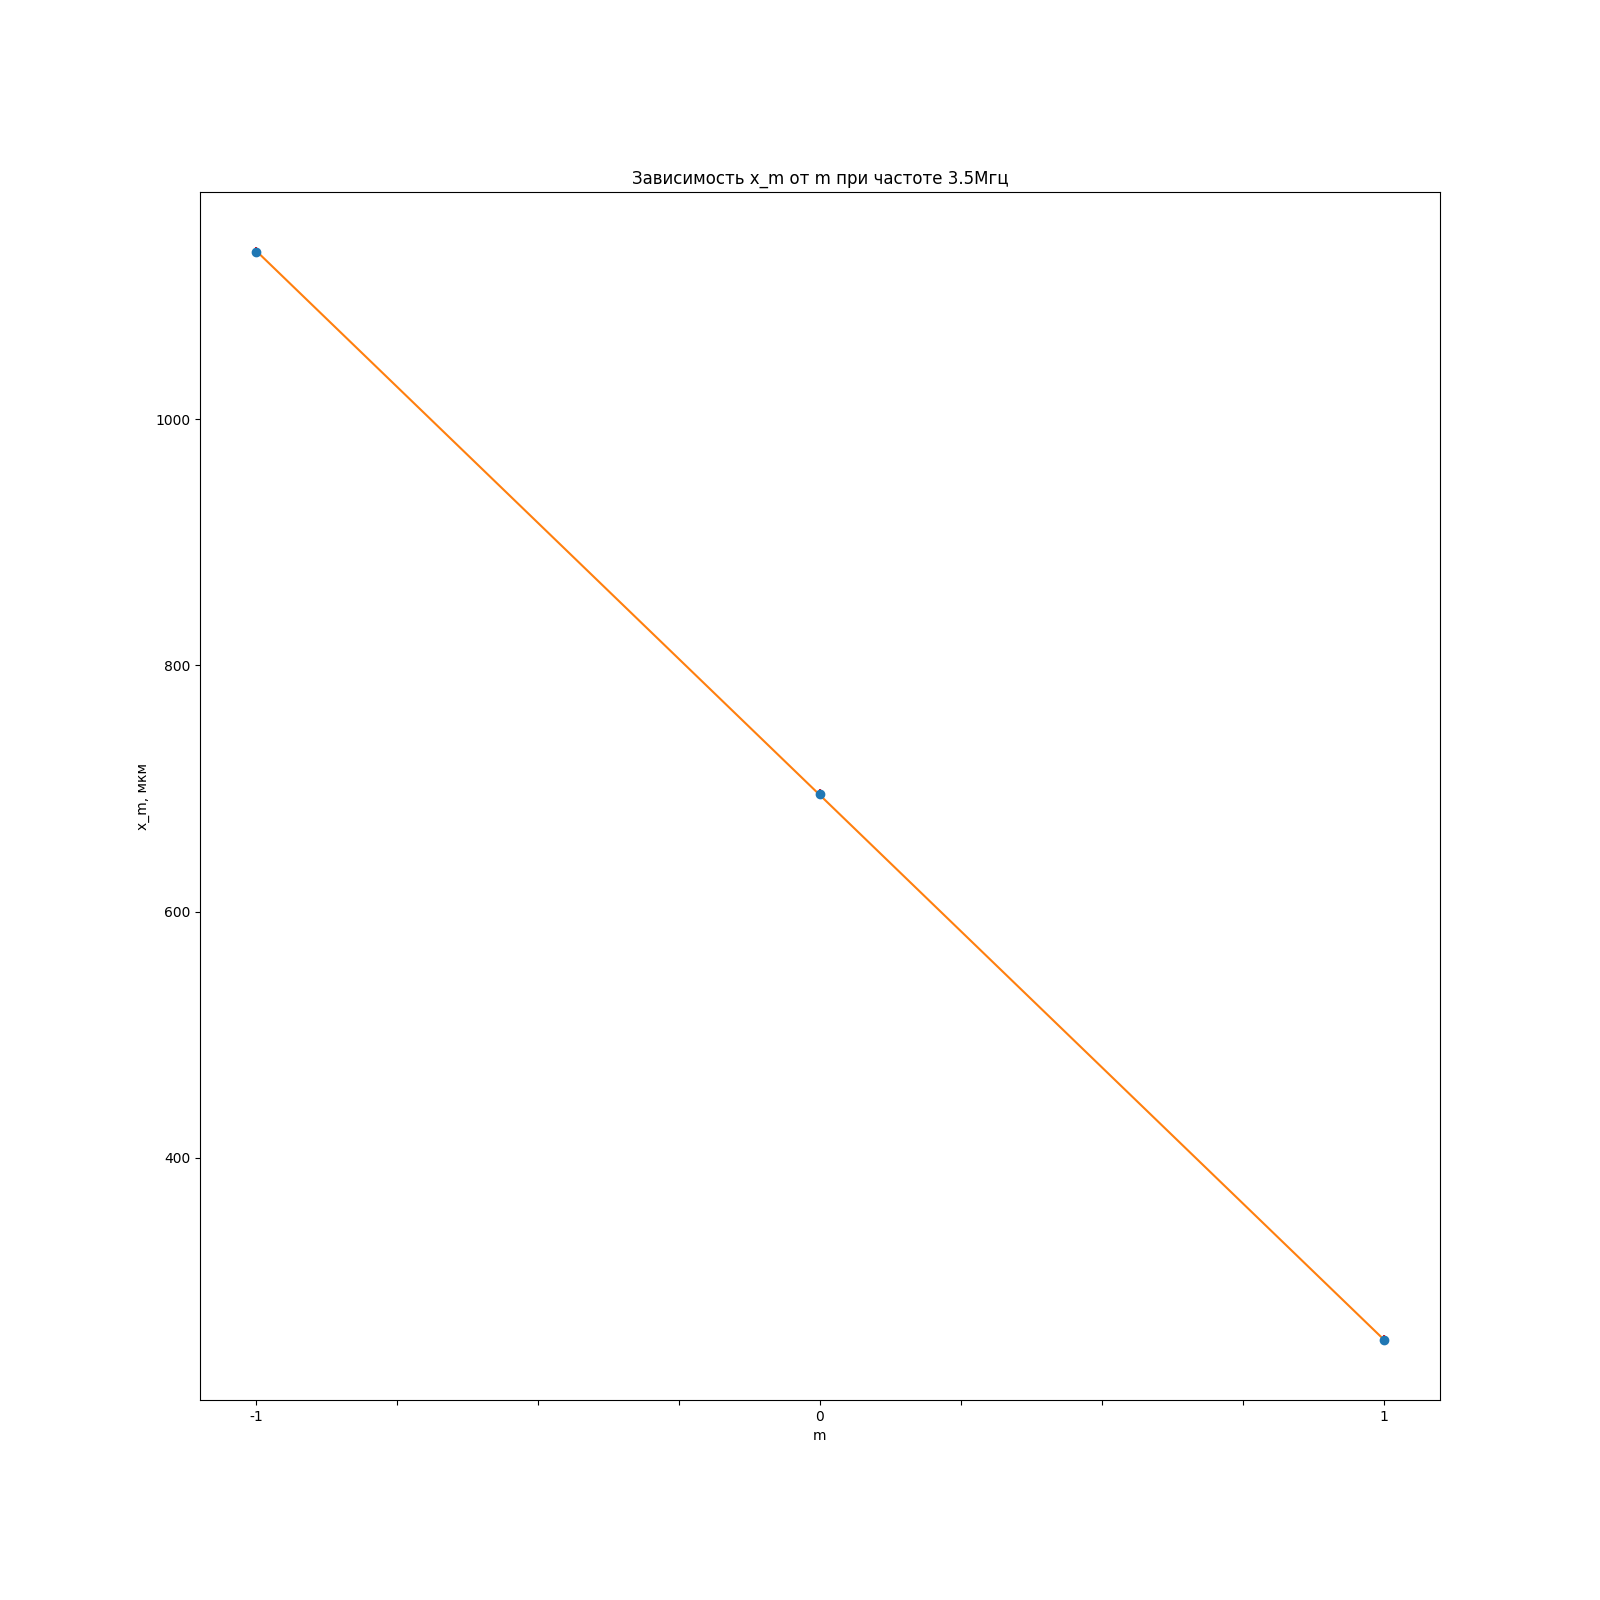
\includegraphics[scale = 0.4]{graph4.png}
        \caption{$f~=~3.5$ МГц}
        \label{g4}
    \end{figure}
\end{document}